%   % !TEX root = ../../VIII,3_Rahmen-TeX_8-1.tex
%
%
%   Band VIII, 3 N.~??A39/Y.8
%   Signatur/Tex-Datei: LH_35_09_14_001-002
%   RK-Nr. 41148
%   Überschrift: De figura trabis ubique aequaliter resistentis
%   Modul: Mechanik / Festigkeit
%   Datierung: [März/April 1683 bis erste Hälfte 1684 (?)]
%   WZ: LEd-Wz 803006 = RK-Wz 273 (Osterode, 1683-1686)
%   SZ: (keins)
%   Bilddateien (PDF): LH_35_09_14_001-002_d1; LH_35_09_14_001-002_d2 (insgesamt: zwei)
%
%
\selectlanguage{ngerman}%
\frenchspacing%
\begin{ledgroupsized}[r]{120mm}%
\footnotesize%
\pstart%
\noindent\textbf{Überlieferung:}%
\pend%
\end{ledgroupsized}%
\begin{ledgroupsized}[r]{114mm}%
\footnotesize%
\pstart%
\parindent -6mm%
\makebox[6mm][l]{\textit{L}}%
Aufzeichnung: LH~XXXV~9,~14 Bl.~1\textendash2.
Ein Bogen~4\textsuperscript{o}.
Dreieinhalb Seiten;
untere Hälfte von Bl.~2~v\textsuperscript{o}\! leer.
% Überschrift auf Bl.~1~r\textsuperscript{o} und Bl.~2~r\textsuperscript{o} nachträglich ergänzt.
Auf Bl.~1~v\textsuperscript{o}\! quer ist folgende Überschrift von Leibnizens Hand aus früherer Verwendung anzutreffen:
\textit{Überschlag der Kosten zu einer} \lbrack/\rbrack\ \textit{Neüen Horizontal WindKunst mit} \lbrack/\rbrack\ \textit{schirmenden Windfängen}
\pend
\end{ledgroupsized}
%
%
\selectlanguage{latin}%
\frenchspacing%
%
%
\vspace{8mm}
\pstart 
\noindent [1~r\textsuperscript{o}]
\pend
\count\Bfootins=1100
\count\Afootins=1100
\count\Cfootins=1100
\pstart
\centering
\edtext{De Figura Trabis ubique aequaliter resistentis.%
\protect\index{Sachverzeichnis}{trabs ubique aequiresistens}%
\protect\index{Sachverzeichnis}{figura trabis}}{%
\lemma{De}\Bfootnote{%
\hspace{-0,5mm}Figura Trabis
\textbar~ubique \textit{erg.}~%
\textbar\ aequaliter resistentis.
\textit{erg.~L}}}%
\edtext{}{\lemma{\textit{Am linken Rand:}}\Afootnote{%
$\astrosun$\newline}}%
\edtext{}{\lemma{\textit{Am oberen Rand:}}\Afootnote{%
Notanda haec methodus\protect\index{Sachverzeichnis}{methodus notandus}
item exemplum\protect\index{Sachverzeichnis}{exemplum}
problematis differentialis determinati.\vspace{-4mm}%
\protect\index{Sachverzeichnis}{problema differentiale determinatum}}}%
\pend
\count\Bfootins=1000
\count\Cfootins=1000
%
\pstart
\vspace{0.5em}% PR: nur provisorisch
\noindent
% \edtext{}{\lemma{}\Bfootnote{Notanda [...] determinati \textit{erg.~L}}}
% \pend
% \pstart
Tandem\edlabel{LH_35_09_14_001-002_ersteUntersuchung-1}
reperi solutionem problematis perdifficilis:%
\protect\index{Sachverzeichnis}{solutio problematis}%
\protect\index{Sachverzeichnis}{problema perdifficile}%
\protect\index{Sachverzeichnis}{quaestio praeparatoria}%
\textso{ quaestio prima praeparatoria }haec est:
% \pend%
% \pstart%
Quaeritur qualis debeat
%
\edtext{esse figura\protect\index{Sachverzeichnis}{figura trabis}
\edtext{Trabis \lbrack\textit{AGCBA}\rbrack}{\lemma{Trabis \lbrack\textit{AGCBA}\rbrack}\Cfootnote{%
Siehe das Diagramm \lbrack\textit{Fig.~1}\rbrack\ auf S.~\pageref{LH_35_09_14_001r_Fig.1}.}}}{%
\lemma{esse}\Bfootnote{%
\textit{(1)}~figura
\textit{(2)}~linea \textit{A}
\textit{(3)}~figura Trabis
\textbar~\textit{AGCA} \textit{ändert Hrsg.}~\textbar%
~\textit{L}}}
%
ita ut proprio\protect\index{Sachverzeichnis}{pondus trabis}
\edtext{pondere non frangatur.}{%
\lemma{pondere}\Bfootnote{%
\textit{(1)}~sustineatur
\textit{(2)}~non frangatur.%
~\textit{L}}}
%
 %[Korr mit anderer Tinte]
%
\edtext{Debet momentum trabis\protect\index{Sachverzeichnis}{momentum trabis}}{%
\lemma{Debet}\Bfootnote{%
\hspace{-0,5mm}\textbar~ergo \textit{gestr.}~%
\textbar\ momentum%
~\textit{L}}}
%
esse
%
\edtext{ubique}{%
\lemma{ubique}\Bfootnote{%
\textit{erg.~L}}}
%
resistentiae\protect\index{Sachverzeichnis}{resistentia trabis}
proportionale.\protect\index{Sachverzeichnis}{momentum resistentiae proportionale}
Est autem resistentia in \textit{FG} ad resistentiam in \textit{BA}%
\protect\index{Sachverzeichnis}{resistentia trabis}
ut quadratum \textit{FG} ad quadratum \textit{BA},
per alibi\edlabel{LH35_09_14_001r_alibiostensa_jfhe-1}
%
\edtext{}{{\xxref{LH35_09_14_001r_alibiostensa_jfhe-1}{LH35_09_14_001r_alibiostensa_jfhe-2}}%
{\lemma{alibi ostensa}\Cfootnote{% Siehe 
N.~14\textsubscript{1}, S.~\refpassage{LH_37_03_073v_ratioquadratorum_tzoiu-1}{LH_37_03_073v_ratioquadratorum_tzoiu-2};
N.~14\textsubscript{2}, S.~\refpassage{LH_37_03_069v_ratioquadratorum-1}{LH_37_03_069v_ratioquadratorum-2}; \refpassage{LH_35_09_16_001r_ratioquadratorum_earjzt-1}{LH_35_09_16_001r_ratioquadratorum_earjzt-2};
N.~14\textsubscript{6}, S.~\refpassage{dnrs_AE_1684_323-324_estenim_jrh-1}{AE_1684_319-325_a4}.}}}% 
%
\edtext{ostensa.\edlabel{LH35_09_14_001r_alibiostensa_jfhe-2}
Ergo portionis trabis \textit{CFGC}
momentum ex \textit{FG} debet esse
ad integrae trabis \textit{CBAC}
momentum ex \textit{BA},}{%
\lemma{ostensa.}\Bfootnote{%
\textit{(1)}~At
\textit{(2)}~Ergo
\textit{(a)}~momentum portionis trabis \textit{CFGC} ad mom
\textit{(b)}~portionis trabis \lbrack...\rbrack\ momentum ex \textit{BA},%
~\textit{L}}}
%
etiam ut quadrat.
\textit{FG} ad quadratum \textit{BA}, quaeritur linea 
%
\edtext{\textit{AGC}.
%
\edlabel{LH_35_09_14_001r_summasummarum_ouir-1}%
Portionis \textit{CFGC} momentum ex \textit{FG}
(\protect\vphantom)%
si \textit{CF} vocetur \textit{x} et \textit{FG} \textit{y}, positis \textit{x} aequidifferentibus%
\protect\vphantom()
erit}{%
\lemma{\textit{AGC}.}\Bfootnote{%
\textit{(1)}~Momentum trabis
\textit{(2)}~Portionis \textit{CFGC} momentum ex \textit{FG}
\textit{(a)}~habetur, si
\textit{(b)}~habetur,
\textit{(c)}~(\protect\vphantom)si \textit{CF}
\textit{(aa)}~vocamus \textit{x}
\textit{(bb)}~vocetur \textit{x} \lbrack...\rbrack\ aequidifferentibus\protect\vphantom() % et \textit{FG} \textit{y}, positis \textit{x}
\textit{(aaa)}~scribi
\textit{(bbb)}~erit%
~\textit{L}}}
%
$\!\!\displaystyle\iint\!\!\! y$ seu summa summarum ipsarum \textit{x}.%
\protect\index{Sachverzeichnis}{summa summarum}%
\edlabel{LH_35_09_14_001r_summasummarum_ouir-2}
%
Debet ergo $\!\!\displaystyle\iint\!\!\! y$ aequ. \textit{byy}.
Sit \textit{y} aequ. $x^e$
et \textit{byy}  aequ. $b \cdot x^{\uline{2e}}$
et
%
\edtext{$\!\!\displaystyle\int\!\!\! y$ aequ. $x^{\uline{e+1}} : \overline{e+1}$}{%
\lemma{$\!\!\displaystyle\int\!\!\! y$ aequ.}\Bfootnote{%
\textit{(1)}~$\dfrac{x^{\uline{e+1}}}{e+1}$
\textit{(2)}~$x^{\uline{e+1}} : \overline{e+1}$%
~\textit{L}}}
%
et
$\!\!\displaystyle\iint\!\!\! y$ aequ. $x^{\uline{e+2}} : \overline{\overline{e+1} \cdot \overline{e+2}}.$%
\rule[-2mm]{0mm}{6mm}
Ergo
$x^{\uline{e+2}} : \overline{\overline{e+1} \cdot \overline{e+2}}$
\pend
\newpage
\centerline{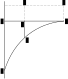
\includegraphics[width=0.42\textwidth]{gesamttex/edit_VIII,3/images/LH_35_09_14_001-002_d1.pdf}}%
  \vspace{0em}
  \centerline{\lbrack\textit{Fig.~1}\rbrack}%
  \label{LH_35_09_14_001r_Fig.1}%
  \vspace{1.5em}%
%  \newpage%
\count\Bfootins=1100
\count\Cfootins=1100
\pstart
\noindent  aequ. \edtext{$b \cdot x^{\uline{2e}}.$
Quae aequatio dividatur in duas,\protect\index{Sachverzeichnis}{aequatio divisa}
$x^{\uline{e+2}}$ aequ. $x^{2e},$}{%
\lemma{$b \cdot x^{\uline{2e}}.$}\Bfootnote{%
\textit{(1)}~Ergo debet fieri $x^{e+2}$ aequ $x^{2e}$
\textit{(2)}~Quae aequatio \lbrack...\rbrack\ duas, $x^{\uline{e+2}}$ aequ. $x^{2e},$%
~\textit{L}}} et
1 aequ. $b \cdot \overline{e+1} \cdot \overline{e+2},$
fiet:
$e+2$ aequ. $2e$
seu
\textit{e} aequ. 2,
\edlabel{LH_35_09_14_001_parabola_fiezv-1}%
\rule[-2mm]{0mm}{6mm}ergo fiet \textit{y}
aequ. $x^2$
seu curva\protect\index{Sachverzeichnis}{curva} \textit{AGC}
est parabola,\protect\index{Sachverzeichnis}{parabola}
cujus vertex \textit{C},
tangens verticis\protect\rule[-3mm]{0mm}{8mm} 
%
\edtext{\textit{CB},
et \textit{b} aequ $\dfrac{1}{12}$
posito latere recto unitate.%
\edlabel{LH_35_09_14_001_parabola_fiezv-2}%
\edlabel{LH_35_09_14_001-002_ersteUntersuchung-2}%
}{%
\lemma{\textit{CB},}\Bfootnote{%
\textit{(1)}~6
\textit{(2)}~et \textit{b} aequ.
\textit{(a)}~6
\textit{(b)}~$\dfrac{1}{12}$
\textit{(3)}~et \textit{b} aequ. \lbrack...\rbrack\ recto unitate.% $\dfrac{1}{12},$ posito latere
~\textit{L}}}%
%
\pend
%
%
%%  \newpage% 
%  \vspace{1.5em}%	% Diagramm Fig.~1
%  \centerline{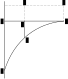
\includegraphics[width=0.40\textwidth]{gesamttex/edit_VIII,3/images/LH_35_09_14_001-002_d1.pdf}}%
%  \vspace*{-1.0em}
%  \centerline{\lbrack\textit{Fig.~1}\rbrack}%
%  \label{LH_35_09_14_001r_Fig.1}%
%  \vspace{1.5em}%
%%  \newpage%
%
%
\pstart%
Atque\edlabel{LH_35_09_14_001-002_zweiteUntersuchung-1}
hanc quidem solutionem\protect\index{Sachverzeichnis}{solutio} facile reperi.
Sed sequitur\textso{ altera quaestio,}
non paulo difficilior.\protect\index{Sachverzeichnis}{quaestio altera}
Ponatur eadem Trabs onere gravata \textit{BD},%
\protect\index{Sachverzeichnis}{trabs onere gravata}
aequaliter per eam diffuso\lbrack;\rbrack\
quaeritur quae tunc figura trabis\protect\index{Sachverzeichnis}{figura trabis} esse debeat,
seu linea \textit{AGC},
ut 
%
\edtext{ubique}{%
\lemma{ubique}\Bfootnote{%
\textit{erg.~L}}}
%
aequaliter resistat\protect\index{Sachverzeichnis}{trabs ubique aequiresistens}
et suo oneri\protect\index{Sachverzeichnis}{onus trabis}
et ponderi imposito.\protect\index{Sachverzeichnis}{pondus impositum}
Sunt enim trabes comparatae non tantum ut se,
sed et ut alias res ferant.\protect\index{Sachverzeichnis}{trabs onere gravata}
\textit{DC} sit \textit{a}.
Ponatur materia\protect\index{Sachverzeichnis}{materia oneris}
%
\edtext{oneris
seu gravitas ejus specifica\protect\index{Sachverzeichnis}{gravitas specifica}
eadem quae trabis
(\protect\vphantom)%
nam si alia sit facilis comparatio est%
\protect\vphantom().
Tunc oneris \textit{CE} momentum%
\protect\index{Sachverzeichnis}{momentum oneris}}{%
\lemma{oneris}\Bfootnote{%
\textit{(1)}~\textbar~seu gravitas ejus specifica \textit{erg.}~%
\textbar\ eadem quae trabis\protect\index{Sachverzeichnis}{gravitas specifica trabis}
(\protect\vphantom)nam si alia sit facilis nihilominus comparatio est%
\protect\vphantom() erit mom
\textit{(2)}~seu gravitas \lbrack...\rbrack\ \textit{CE} momentum%
~\textit{L}}}
%
ex \textit{EG} est $\dfrac{1}{2}axx.$
Ergo totius trabis\protect\index{Sachverzeichnis}{momentum trabis}
et 
%
\edtext{oneris \textit{CDEGC}\protect\index{Sachverzeichnis}{momentum oneris}
momentum totum}{%
\lemma{oneris}\Bfootnote{%
\textit{(1)}~momentum simul
\textit{(2)}~\textit{CDEGC} momentum totum%
~\textit{L}}}
%
ex \textit{EG} est \protect\rule[-2mm]{0mm}{7mm}$\!\!\displaystyle\iint\!\!\! y+\dfrac{1}{2}axx$
quod debet esse proportionale resistentiae,%
\protect\index{Sachverzeichnis}{resistentia trabis}%
\rule[0mm]{0mm}{4mm}
ut \textit{yy}
quae est in sola trabe circa \textit{FG},
et erit $\!\!\displaystyle\iint\!\!\! y+\dfrac{1}{2}axx$ aequ. \textit{byy}.
%
\lbrack1~v\textsuperscript{o}\rbrack\ %%%% Blatt 1v
%
% \pend
% %
% %
% \pstart
\rule[0mm]{0mm}{5mm}%
Hanc aequationem differentialem\protect\index{Sachverzeichnis}{aequatio differentialis}
calculo\protect\index{Sachverzeichnis}{calculus} in omnem partem
\pend
\newpage
\pstart
\noindent versavi,
donec solutionem\protect\index{Sachverzeichnis}{solutio}
tali methodo\protect\index{Sachverzeichnis}{methodus} reperi
qua nunquam antea usus eram,
licet seriebus infinitis,\protect\index{Sachverzeichnis}{series infinita}
quibus ad eam perveni,
dudum essem usus.
Ponatur\edlabel{LH35_09_14_001v_1}
%
% \edtext{}{{\xxref{LH35_09_14_001v_1}{LH35_09_14_001v_2}}%
% {\lemma{Ponatur}\Bfootnote{%
% \textit{(1)}~\textit{y} aequ $l+mx+nxx+px^3+qx^4$ etc. fit $\!\!\displaystyle\iint\!\!\! y$ aeq. 
% \textit{(2)}~\textit{y} aequ. \textit{L}}}}
%
% [folgendes tabellarisch]
\pend
\vspace{0.5em}%
\pstart%
\label{KZeitz87}%
\centering%
\renewcommand{\arraystretch}{1.5}%
$\setlength{\arraycolsep}{3pt}%
\begin{array}{lrcrcrcrcrcrcrcll}%
%\edlabel{LH_35_09_14_001r_erstetabelle_kduag-1}%
& y & \text{aequ.} & l & + & mx & + & nxx & + & px^3 & + & qx^4 & + & rx^5 & \text{etc.} & & \\
& \raisebox{6pt}{\makebox[30pt][l]{\uline{\makebox[300pt][l]{}}}} & & & & & & & & & & & & & & & \\
\text{fiet}\qquad &\!\!\displaystyle\iint\!\!\! y & \text{aequ.}\edlabel{LH35_09_14_001v_2} & & & & & \dfrac{1}{2}lxx & + & \dfrac{1}{6}mx^3 & + & \dfrac{1}{12}nx^4 & + & \dfrac{1}{20}px^5 & \text{etc.} & & \\
\rule[0mm]{0mm}{7mm}%
& +\, \dfrac{1}{2}axx & \text{aequ.} & & & & & \dfrac{1}{2}axx & & & & & & & \text{etc.} & & \\
&\text{a\,e\,q\,u\,.} & & & & & & & & & & & & & & & \\
&byy & \text{aequ.} & ll & + & 2lmx & + &2lnxx & + & 2lpx^3 & + & 2lqx^4 & + & 2lrx^5 & \text{etc.} & &
\parbox[t][-13pt][c]{0pt}{$\left. \vphantom{\begin{array}{l} 0\\0\\0\\0\\0\\0\\0\end{array}}\right \} \astrosun$}\label{LH_35_09_14_001v_auringonmerkki} %  %  %  %  %  %  %  %  %  %  %  %  %  %  %  %  %  %  %  %  %  %  %
\\
& & & & & & + & mm\makebox[0pt][l]{\,$\cdot$\,$\cdot$}\phantom{xx} & & 2mn\makebox[0pt][l]{\,$\cdot$\,$\cdot$}\phantom{x^3} & &2mp\makebox[0pt][l]{\,$\cdot$\,$\cdot$}\phantom{x^4} & & 2mq\makebox[0pt][l]{\,$\cdot$\,$\cdot$}\phantom{x^5} & \text{etc.} &
\parbox[b][-15pt][c]{15pt}{$\left. \vphantom{\begin{array}{l} 0\\0\\0\\0\end{array}}\right \} [b]$} & %  %  %  %  %  %  %  %  %  %  %  %  %  %  %  %  %  %  %  %  %  %  %
\\
& & & & & & & & & & & nn\makebox[0pt][l]{\,$\cdot$\,$\cdot$}\phantom{x^4} & & 2np\makebox[0pt][l]{\,$\cdot$\,$\cdot$}\phantom{x^5} & \text{etc.} & & \\
& & & & & & & & & & & & & & \text{etc.} & &
%\edlabel{LH_35_09_14_001r_erstetabelle_kduag-2}%
\end{array}$
%
\edtext{}{\lemma{\hspace{1.6mm}7--10 \hspace{1,6mm}$\displaystyle ll + 2lmx + 2lnxx$ \lbrack...\rbrack\ $2np$ etc. etc.\,}\killnumber\Cfootnote{%
Der gemeinsame Faktor \textit{b} in den letzten vier Zeilen der tabellarischen Darstellung und die entsprechende geschweifte Klammer sind vom Hrsg. ergänzt.
In der tabellarischen Darstellung auf S.~\pageref{KZeitz88} wird der Faktor \textit{b} durch einen äquivalenten Faktor \textit{c} ersetzt.}}%
% y aequ l+mx+nxx+px^3+qx^4+rx^5 etc. [darunter Abtrennungslinie]
% \int\int y aequ ——— \frac ½lxx+\frac 1/6mx^3+\frac 1/12nx^4+\frac 1/20px^5 etc.
% <aequ>
% +\frac ½axx aequ. ——— \frac ½axx 						etc.
% aequ 
% byy aequ 	ll	+<mx>{2lmx}	+{2}<n>{l}nxx	+2lpx^3	+2lqx^4+2lrx^5 etc
%					+mm..		2mn..       2mp      2mq..  etc
%							                 nn         2np      etc
%										etc
% [über die Zeilen unter dem Abtrennungsstrich rechts geschweifte Klammer mit Verweiszeichen astrosun]
%
% $\blacksquare\blacksquare$ [Faktor \textit{b} fehlt in den Z. 5$-$7 auf der r. Seite]
\pend%
 \vspace{1.0em}%
%
\pstart%
\noindent%
\setline{11}Et 
%
\edtext{totam aequationem}{%
\lemma{totam}\Bfootnote{%
\textit{(1)}~quantitatem
\textit{(2)}~aequationem%
~\textit{L}}}
%
$\astrosun$ faciendo identicam,%
\protect\index{Sachverzeichnis}{aequatio identica}
ita ut indeterminata \textit{x} in ea evanescat,
fiet:
%
\edtext{\textit{l} aequ. 0, et}{%
\lemma{\textit{l} aequ. 0}\Bfootnote{\hspace{-0,5mm}%
\textit{(1)}~\textit{m} aequ
\textit{(2)}~et%
~\textit{L}}}
% 
quidem si abesset litera ${a}$\protect\index{Sachverzeichnis}{litera}
seu \protect\rule[-2mm]{0mm}{7mm}quantitas $\dfrac{1}{2}axx,$
liceret omnes literas ponere aequales nihilo,\protect\index{Sachverzeichnis}{nihilum}
servata sola litera \textit{n},
\edlabel{LH_35_09_14_001v_bSetzung-1}%
et \protect\rule[-4mm]{0mm}{8mm}fieret \textit{n} aequ. $\dfrac{1}{12b}$
et \textit{y} aequ
%
\edtext{$\dfrac{1}{12b}xx$ seu \textit{y} aequ. \textit{xx},
si \textit{b} aequ. $\dfrac{1}{12},$%
\edlabel{LH_35_09_14_001v_bSetzung-2}
et}{%
\lemma{$\dfrac{1}{12b}xx$}\Bfootnote{%
\textit{(1)}~et rediret seu
\textit{(2)}~seu \textit{y} aequ. \textit{xx}, si \textit{b} aeq. $\dfrac{1}{12}$
\textit{(3)}~seu \textit{y} aequ. \textit{xx},
\textit{(a)}~\textbar~si \textit{streicht Hrsg.}~\textbar\ \textit{b} aequ. $\dfrac{1}{12}$
\textit{(b)}~si \textit{b} aequ. $\dfrac{1}{12},$ et%
~\textit{L}}}
%
haberetur hac methodo\protect\index{Sachverzeichnis}{methodus}
%
\edtext{parabola\protect\index{Sachverzeichnis}{parabola}
quae
\edtext{supra,}{%
\lemma{supra}\Cfootnote{%
S.~\refpassage{LH_35_09_14_001_parabola_fiezv-1}{LH_35_09_14_001_parabola_fiezv-2}.}}
si}{%
\lemma{parabola}\Bfootnote{%
\textit{(1)}~, si \textit{a}
\textit{(2)}~, et
\textit{(3)}~quae supra, si%
~\textit{L}}}
%
solum pondus trabis\protect\index{Sachverzeichnis}{pondus trabis} consideraretur.
Sed quia
debet 
%
\edtext{(ob onus impositum)\protect\index{Sachverzeichnis}{onus trabi impostitum}}{%
\lemma{(\protect\vphantom)ob}\Bfootnote{%
\hspace{-0,5mm}onus impositum\protect\vphantom()
\textit{erg.~L}}}
%
 \protect\rule[-2.5mm]{0mm}{8mm}conservari \textit{m},
et fieri aequ.
%\pend%%%%%%%%%%%%%%%%Künstlicher Seitenumbruch KZEITZ
%\newpage
%\pstart
%\noindent 
$\sqrt{\dfrac{1}{2}a:b},$
\makebox[1.0\textwidth][s]{hinc video eidem methodo\protect\index{Sachverzeichnis}{methodus} insistendo feliciter evenire,
ut omnes \protect\rule[-2.0mm]{0mm}{6mm}literae\protect\index{Sachverzeichnis}{litera}
possint poni}
\pend
\newpage
\pstart
\noindent aequales nihilo,\protect\index{Sachverzeichnis}{nihilum}
demtis \textit{m} et \textit{n}.
%
\edtext{Nam quaerendo \textit{n}, per gradum $x^3,$%
\protect\index{Sachverzeichnis}{gradus}}{%
\lemma{Nam}\Bfootnote{\hspace{-0,5mm}%
\textbar~ponendo \textit{m} aequ $\sqrt{\dfrac{1}{2}a},$ et \textit{gestr.}~%
\textbar\ quaerendo \textit{n},
\textbar~(\protect\vphantom)posita \textit{l} aequ. 0\protect\vphantom() \textit{gestr.}~%
\textbar\ per gradum $x^3,$%
~\textit{L}}}
%
oritur aequatio comparatitia\protect\index{Sachverzeichnis}{aequatio comparatitia}
$\dfrac{1}{6}m$ aequ. $2bmn,$
seu
\textit{n} aequ. $\dfrac{1}{12b},$ % Vorlage: $\dfrac{1}{12b}.$
 \protect\rule[-2.0mm]{0mm}{6mm}ut in gradu $x^4$\protect\index{Sachverzeichnis}{gradus}
caeteris destructis fit
$\dfrac{1}{12} n$ aequ. \textit{bnn}
seu rursus
\textit{n} aequ. $\dfrac{1}{12b}.$
Itaque faciemus
\textit{y} aequ. $x\sqrt{\dfrac{1}{2}a:b}+\dfrac{1}{12b}xx$ 
%
\edtext{seu \textit{y} aequ. $x\sqrt{6a}+xx$}{%
{\lemma{seu}\Bfootnote{%
\textit{y} aequ. $x\sqrt{6a}+xx$
\textit{erg.~L}}}%
{\lemma{seu \textit{y} aequ. $x\sqrt{6a}+xx$}\Cfootnote{%
Die Folgerung beruht auf der früheren Setzung $\displaystyle b = \frac{1}{12};$
vgl. S.~\refpassage{LH_35_09_14_001v_bSetzung-1}{LH_35_09_14_001v_bSetzung-2}.}}}
%
quae aequatio satisfaciet quaesito.%
\protect\index{Sachverzeichnis}{aequatio satisfaciens quaesito}%
\protect\index{Sachverzeichnis}{quaesitum}
Itaque curva\protect\index{Sachverzeichnis}{curva} \textit{AGC} rursus
%
\edtext{parabola\protect\index{Sachverzeichnis}{parabola} erit,
verum}{%
\lemma{parabola}\Bfootnote{%
\hspace{-0,5mm}erit,
\textit{(1)}~sed
\textit{(2)}~verum%
~\textit{L}}}
%
\textit{C} non erit curvae vertex,%
\protect\index{Sachverzeichnis}{vertex curvae}
\textit{AB} tamen ut ante ejus axi\protect\index{Sachverzeichnis}{axis curvae}
%
\edtext{parallela erit,
descriptio\protect\index{Sachverzeichnis}{descriptio curvae}}{%
\lemma{parallela}\Bfootnote{%
\hspace{-0,5mm}erit,
\textit{(1)}~determinatio
\textit{(2)}~descriptio%
~\textit{L}}}
%
autem curvae ex his non erit difficilis.%
\edlabel{LH_35_09_14_001-002_zweiteUntersuchung-2}
\pend%
%
% [Einfügung quer auf dem Blatt] 
%S
\pstart%
Video\edlabel{LH_35_09_14_001v_quer_uzvfk-1}%
\edtext{}{%
{\xxref{LH_35_09_14_001v_quer_uzvfk-1}{LH_35_09_14_001v_quer_uzvfk-2}}%
{\lemma{Video}\Bfootnote{%
\hspace{-0,5mm}etiam \lbrack...\rbrack\ % fieri posset, si
% \textbar~aliud \textit{ändert Hrsg.}~% \textbar\ adhuc curva 
ubi \textit{x}
\textbar~ingredereretur \textit{ändert Hrsg.}~%
\textbar\ irrationalem vel fractam locum haberet.
\textit{erg.~L}}}}
%
etiam ne posse quidem aliam reperiri curvam,%
\protect\index{Sachverzeichnis}{curva}\protect\index{Sachverzeichnis}{parabola}
et problema esse determinate solutum.%
\protect\index{Sachverzeichnis}{problema determinate solutum}
Nam valor\protect\index{Sachverzeichnis}{valor}
ipsius \textit{m} et \textit{n} se sponte offert,
et \textit{l} fit $0$
et ex gradu $x^4,$\protect\index{Sachverzeichnis}{gradus}
substituto ibi valore ipsius \textit{n},
fit \textit{p} etiam $0.$
Ergo et \textit{q} ob $x^5,$
et ita porro reliquae literae omnes.\protect\index{Sachverzeichnis}{litera}
\edtext{Utile est aequationes differentiales\protect\index{Sachverzeichnis}{aequatio differentialis}
mutare in summatorias,\protect\index{Sachverzeichnis}{aequatio summatoria}
ut fiant determinatae.\protect\index{Sachverzeichnis}{aequatio determinata}}{%
\lemma{\textit{Auf}}\Afootnote{%
\hspace{-0,5mm}Utile est \lbrack...\rbrack\ fiant determinatae \textit{bezogen:}
\textso{NB NB}\newline}}
% \pend
% \pstart
% NB NB
% \pend
% \pstart
Itaque \textit{y} non potest exprimi per \textit{x}
aequatione infinita,\protect\index{Sachverzeichnis}{aequatio infinita}
quod fieri posset,
si aliud % \lbrack alia\rbrack\ 
adhuc curva\protect\index{Sachverzeichnis}{curva}
ubi \textit{x}
%
\lbrack ingrederetur\rbrack\
%
\edtext{irrationalem vel fractam}{%
\lemma{irrationalem vel fractam}\Cfootnote{%
Gemeint ist \textit{aequationem}.}}
%
locum haberet.%
\edlabel{LH_35_09_14_001v_quer_uzvfk-2}
\pend
\pstart
Hic ergo rursus usus sum illo artificio inveniendi a me%
\protect\index{Sachverzeichnis}{artificium inveniendi}
%
\edtext{alias}{%
\lemma{alias}\Cfootnote{Nicht nachgewiesen.}}
%
annotato duplicis methodi.\protect\index{Sachverzeichnis}{methodus duplex}
Nempe si problema difficile\protect\index{Sachverzeichnis}{problema difficile}
aliqua methodo
quae mihi ad ipsum solvendum apta 
%
\edtext{videtur,
quaerere velim,}{%
\lemma{videtur,}\Bfootnote{%
\textit{(1)}~velim
\textit{(2)}~quaerere velim%
~\textit{L}}}
prius eadem methodo quaero
problema aliquod facile\protect\index{Sachverzeichnis}{problema facile}
notae ex alia 
%
\edtext{faciliore\protect\index{Sachverzeichnis}{methodus facilis}}{%
\lemma{faciliore}\Bfootnote{%
\textit{erg.~L}}}
%
methodo solutionis,\protect\index{Sachverzeichnis}{solutio nota}
et video quomodo ipsius solutio ex hac quoque methodo
%
\edtext{difficiliore}{%
\lemma{difficiliore}\Bfootnote{%
\textit{erg.~L}}}
%
derivetur,
ita disco modum utendi methodo hac difficiliore,%
\protect\index{Sachverzeichnis}{methodus difficilis}
et facilius ejus ope ad problema etiam difficile pervenio.%
\protect\index{Sachverzeichnis}{problema difficile}
%
\lbrack2~r\textsuperscript{o}\rbrack\ %%%% Blatt 2r
%
\pend
% \vspace{1.0em}%
\newpage%
%
\pstart%
% \centering
%
% \edtext{}{%
% \lemma{De}\Bfootnote{%
% \hspace{-0,5mm}Figura Trabis aequaliter resistentis.
% \textit{erg.~L}}}
%
\edtext{}{\lemma{\textit{Am oberen Rand,}}\Afootnote{%
\hspace{-0,5mm}\textit{nachträglich hinzugefügt:}
De Figura Trabis aequaliter resistentis.%
\protect\index{Sachverzeichnis}{trabs ubique aequiresistens}%
\protect\index{Sachverzeichnis}{figura trabis}
\mbox{Hujus} Schedae\protect\index{Sachverzeichnis}{scheda}
pagina\protect\index{Sachverzeichnis}{pagina}
prima et secunda\textsuperscript{\lbrack a\rbrack} tentavit,
et post frustraneas evagationes\protect\index{Sachverzeichnis}{evagatio frustranea} 
in annotatiuncula\protect\index{Sachverzeichnis}{annotatiuncula}
hujus paginae signo\protect\index{Sachverzeichnis}{signum}
$\astrosun$\textsuperscript{\lbrack b\rbrack} absolvit.
Inventum pagina\protect\index{Sachverzeichnis}{pagina}
tertia et quarta\textsuperscript{\lbrack c\rbrack}
est ordinatum et distincte explicatum.\vspace{0.5em}%
\newline%
{\footnotesize%
\textsuperscript{\lbrack a\rbrack}
pagina prima et secunda:
Bl.1~r\textsuperscript{o} und 1v\textsuperscript{o}
\quad
\textsuperscript{\lbrack b\rbrack}
signo $\astrosun$:
Vgl. S.~\pageref{KZeitz87}.
\quad
\textsuperscript{\lbrack c\rbrack}
pagina tertia et quarta:
Blatt 2~r\textsuperscript{o} und 2v\textsuperscript{o}
\newline%
}}}%
% \pend%
% \vspace*{0.5em}%
%
% \pstart
% \noindent
% Hujus\edlabel{LH35_09_14_002r_1}% 
% %
% \edtext{}{{\xxref{LH35_09_14_002r_1}{LH35_09_14_002r_2}}%
% \lemma{}\Bfootnote{%
% Hujus [...] explicatum. \textit{erg.~L}}}
% Schedae pagina prima et secunda tentavit, et post frustraneas evagationes\protect\index{Sachverzeichnis}{evagatio}
% in annotatiuncula\protect\index{Sachverzeichnis}{annotatiunculum} hujus paginae signo $\astrosun$ absolvit. Inventum 
% %
% \edtext{[pagina]}{%
% \lemma{}\Bfootnote{%
% ppagina \textit{L~ändert Hrsg.}}}
% tertia et quarta
% est ordinatum
% et distincte
% explicatum.\edlabel{LH35_09_14_002r_2}
% \pend
%
% \pstart% 
% \centering%
% \noindent%
Aequatio calculi differentialis:%
\protect\index{Sachverzeichnis}{aequatio calculi differentialis}%
\protect\index{Sachverzeichnis}{calculus differentialis}
\textit{axx} aequ. $cyy-\!\!\!\displaystyle\int\!\!\overline{\!\!\!\!\displaystyle\int\!\!\overline y},$
positis \textit{x} aequidifferentibus.\protect\index{Sachverzeichnis}{aequidifferens}
% [folgendes tabellarisch]
\pend
%\newpage
\pstart
\label{KZeitz88}%
\centering
\renewcommand{\arraystretch}{1.6}
\setlength{\arraycolsep}{0.5pt}
%
$\begin{array}{lccrcrcrcrcrcrcrcrcrll}
%\edlabel{LH_35_09_14_002r_zweitetabelle_gwd-1}%
\text{Sit} & y & \text{aequ.} & l & + & mx & + & nxx & +& px^3 & + & qx^4 & + & rx^5 & + & tx^6 & + & vx^7 & + & zx^8 & &
\parbox[c][12pt][t]{30pt}{$\left. \vphantom{\begin{array}{l} 0\\0\\0\\0\\0\\0\\0\\0\end{array}}\right \} 0$}%  %  %  %  %  %  %  %  %  %  %  %  %  %  %  %  %  %  %  %  %  %  %
\\ 
\text{fiet} & cyy & \text{aequ.} & ll & + & 2lmx & + & 2lnxx & + & 2lpx^3 & + & 2lqx^4 & + & 2lrx^5 & + & 2ltx^6 & + & 2lvx^7 & + & 2lzx^8 & & \\
 & & & & & & & mm\hphantom{xx} & & 2mn\hphantom{x^3} & & 2mp\hphantom{x^4} & & 2mq\hphantom{x^5} & & 2mr\hphantom{x^6} & & 2mt\hphantom{x^7} & & 2mv\hphantom{x^8} & & \\
 & & & & & & & & & & & nn\hphantom{x^4} & & 2np\hphantom{x^5} & & 2nq\hphantom{x^6} & & 2nr\hphantom{x^7} & & 2nt\hphantom{x^8} &
\parbox[c][0pt][c]{20pt}{$\left. \vphantom{\begin{array}{l} 0\\0\\0\\0\\0\end{array}}\right \} c$}& \\%  %  %  %  %  %  %  %  %  %  %  %  %  %  %  %  %  %  %  %  %  %  %
 & & & & & & & & & & & & & & & pp\hphantom{x^6} & & 2pq\hphantom{x^7} & & 2pr\hphantom{x^8} & & \\
 & & & & & & & & & & & & & & & & & & & qq\hphantom{x^8} & & \\
% [über die vorigen 5 Zeilen rechts geschweifte Klammer mit nebenstehendem Faktor c]
 & -\!\!\displaystyle\iint\!\!\!y & & & & & & \dfrac{1}{2}l\phantom{xx} & & \dfrac{1}{6} m\phantom{x^3} & & \dfrac{1}{12} n\phantom{x^4} & & \dfrac{1}{20} p\phantom{x^5} & & \dfrac{1}{30}q\phantom{x^6} & & \dfrac{1}{42} r\phantom{x^7} & & \dfrac{1}{56} t\phantom{x^8} &
\left. \vphantom{\begin{array}{l} 0\end{array}}\right \} -1 & \\%  %  %  %  %  %  %  %  %  %  %  %  %  %  %  %  %  %  %  %  %  %  %
% [rechts der vorigen Zeile geschweifte Klammer mit Faktor -1]
 & \uline{-\,axx} & & & & & & -\,a\phantom{xx} & & & & & & & & & & & & & \\	
% [Summationsstrich unter –axx; rechts der Tabelle ab der fiet-Zeile geschweifte Klammer mit nebenstehender 0]
 & 0 & \text{aequ.} & 0 & + & 0\hphantom{x} & + & 0\hphantom{xx} & + & 0\hphantom{x^3} & + & 0\hphantom{x^4} & + & 0\hphantom{x^5} & + & 0\hphantom{x^6} & + & 0\hphantom{x^7} & + & 0\hphantom{x^8} & & 
\end{array}$%
%\edlabel{LH_35_09_14_002r_zweitetabelle_gwd-2}%
%
\edtext{}{%
% {\xxref{LH_35_09_14_002r_zweitetabelle_gwd-1}{LH_35_09_14_002r_zweitetabelle_gwd-2}}%
{\lemma{\hspace{1,6mm}7 \hspace{1.6mm}\textit{Am Rand,}}\killnumber\Afootnote{%
\hspace{-0,5mm}\textit{an die vorletzte Zeile der tabellarischen Darstellung anschließend:}
Si abesset \textit{a},
possent omnes literae\protect\index{Sachverzeichnis}{litera}
poni aequales nihilo,\protect\index{Sachverzeichnis}{nihilum}
servata sola litera \textit{n}. 
Nunc vero quia\textsuperscript{\lbrack a\rbrack} adest \textit{a}
video rem succedere
positis omnibus literis\protect\index{Sachverzeichnis}{litera}
aequalibus 0 praeter \textit{m} et \textit{n}. 
Et ita solutum est problema.%
\protect\index{Sachverzeichnis}{problema solutum}
Videatur pagina versa\protect\index{Sachverzeichnis}{pagina}
\protect\index{Sachverzeichnis}{signum}signum $\astrosun.$\textsuperscript{\lbrack b\rbrack}\vspace{0.5em}%
\newline %
{\footnotesize%
\textsuperscript{\lbrack a\rbrack} quia \textit{(1)}~abest \textit{(2)}~adest \textit{L}
\quad
\textsuperscript{\lbrack b\rbrack}
signo $\astrosun$:
Vgl. S.~.~\pageref{KZeitz87}.\vspace{-3mm}}}}}%
%
\pend%
\vspace{1.0em}
\newpage%
%
\pstart%
\noindent%
% \rule[0mm]{0mm}{6mm}%
Ergo
\quad%
\textit{l} aequ. 0.
\quad%
\textit{m} aequ. $\sqrt[2]{a : c}.$
%
\quad%
\textit{n} aequ. $+\,\dfrac{1}{2 \cdot 6c}$ 
\pend%
\pstart%
\noindent%
\rule[0mm]{0mm}{6mm}%
\textit{p} aequ. $\dfrac{1}{2 \cdot 2 \cdot 6 \cdot 12\sqrt[2]{ac}} -
\edtext{\dfrac{1}{2 \cdot 2 \cdot 2 \cdot 6 \cdot 6 c \sqrt[2]{ac}}$%
}{%
\lemma{$\dfrac{1}{2 \cdot 2 \cdot 6 \cdot 12\sqrt[2]{ac}}$}\Cfootnote{%
Im Nenner fehlt ein Faktor \textit{c}.
Der Fehler setzt sich fort, weitere kommen hinzu.
Bei korrekter Rechnung verschwinden \textit{p}
und folglich auch alle Koeffizienten der höheren Potenzen der Variabel \textit{x}.
Leibniz hat den Irrtum offensichtlich bemerkt,
wie die Randbemerkung zur tabellarischen Darstellung auf S.~\pageref{KZeitz88} erkennen lässt.}}
%
seu $\dfrac {c-1}{2 \cdot 2 \cdot 2 \cdot 6 \cdot 6 c \sqrt[2]{ac}}$
\pend%
\pstart%
\noindent%
\rule[0mm]{0mm}{6mm}%
\textit{q} aequ. $\dfrac{c-1}{2 \cdot 2 \cdot 2 \cdot 6 \cdot 6 \cdot c\sqrt{ac} \cdot 20 \cdot 2\sqrt{ac}}$
% \edtext{aequ. $\dfrac{c-1}{2 \cdot 2 \cdot 2 \cdot 6 \cdot 6 \cdot c\sqrt{ac} \cdot 20 \cdot 2\sqrt{ac}}$}
% {\lemma{aequ.}\Bfootnote{\textit{(1)}~$\dfrac{1}{20 \cdot 2}p$ \textit{(2)}~$\dfrac{p \blacksquare\blacksquare}
% {20 \cdot 2\sqrt{a:c}} -$ \textit{(3)}~$\dfrac{c-1}{2 \cdot 2 \cdot 2 \cdot 6 \cdot 6 \cdot c\sqrt{ac} \cdot 20 \cdot 2\sqrt{ac}}$ \textit{ L }\ }}
$-\dfrac{c-1}{2 \cdot 2 \cdot 2 \cdot 6 \cdot 6 \cdot c\sqrt{ac} \cdot 2 \cdot 6c \cdot \sqrt{ac} \cdot \sqrt{a:c}}$ 
% [über den Fortsetzungsfehler hinaus im Nenner ein Faktor sqrt{a:c} zuviel]
seu 
\pend%
\pstart%
\noindent%
\rule[0mm]{0mm}{8mm}%
\textit{q} aequ. $\dfrac{3\sqrt{ac}-10\overline{c-1}}{2 \cdot 12^3 \cdot 20cc\sqrt{ac}}.$%
% [weitere Rechenfehler]
\rule[0mm]{0mm}{7mm}%
\pend%
% \newpage%
%
\pstart%
\rule[0mm]{0mm}{4mm}%
Ut progressionem seriei\protect\index{Sachverzeichnis}{progressio seriei}
arte aliqua compendiosa\protect\index{Sachverzeichnis}{ars compendiosa}
inveniamus,
consideremus terminos hos:\protect\index{Sachverzeichnis}{terminus}
\textit{m}. \textit{n}. \textit{p}. \textit{q}. etc.
(\protect\vphantom)%
nam \textit{l} evanescit%
\protect\vphantom()
et terminum
%
\edtext{vocemus $\omega,$ numerum}{%
\lemma{vocemus}\Bfootnote{%
\hspace{-0,5mm} $\omega,$
\textit{(1)}~uno nu
\textit{(2)}~numerum%
~\textit{L}}}
%
terminorum,
qui idem est cum numero exponentium \textit{x},%
\protect\index{Sachverzeichnis}{numerus exponentium}
vocemus \textit{H}.
Et % si ? 
uno termino\protect\index{Sachverzeichnis}{terminus}
\edlabel{LH35_09_14_002r_11}appellato
%
\edtext{}{%
{\xxref{LH35_09_14_002r_11}{LH35_09_14_002r_12}}%
{\lemma{appellato}\Bfootnote{%
\textit{(1)}~$\omega$ proxime sequentem vocemus $(1)\omega$ adhuc sequentem (2)$\omega,$ intervallo numeri terminorum 
\textbar\ computatis extremis \textit{erg.}~%
\textbar\ remotum $(H)\omega,$ intervallo numeri terminorum demto uno remotum $(\overline{H-1})\omega,$ et habebitur aequatio
\textit{(a)}~$\omega$ aequ.
\textit{(b)}~$\dfrac{1}{2c \cdot H \cdot \overline{H+1}}(2)\omega$ aequ. $\omega \cdot (H)\omega + (1)\omega(H-1)\omega+(2)\omega(H-2)\omega$
\textit{(2)}~$(1),$ proxime antecedentem \lbrack...\rbrack\ $(3)(H-2) + (4)(H-3)$%
~\textit{L}}}}%
%
$(1),$ proxime antecedentem vocemus $(2),$
adhuc priorem $(3),$
intervallo numeri terminorum computatis extremis remotum $(H),$
intervallo numeri terminorum\protect\index{Sachverzeichnis}{intervallum numeri terminorum}
dempto uno remotum $(\overline{H-1}),$
et habebitur aequatio
%
$\dfrac{1}{2c \cdot H \cdot H-1}(2)$ aequ. $(1)(H) + (2)(H-1) + (3)(H-2) + 
(4)(H-3)$\edlabel{LH35_09_14_002r_12} 
usque ad $\displaystyle\dfrac{\left(\displaystyle\frac{\overline{H+1}}{2}\right)
\left(\displaystyle\frac{\overline{H+1}}{2}\right)}{2}$
%
verbi gratia:\rule[-4mm]{0pt}{16,0mm}
%
$\dfrac{1}{2c \cdot 8 \cdot 7}t$\, aequ. $vm + tn + rp$ etc. … $\dfrac{qq}{2}.$
%
\lbrack2~v\textsuperscript{o}\rbrack\ %%%% Blatt 2v
%
\pend
\vspace{2mm}
%
%
\pstart
\edtext{Mirabile genus%
\protect\index{Sachverzeichnis}{genus seriei mirabile}}{%
\lemma{Mirabile}\Bfootnote{%
\textit{(1)}~terminus
\textit{(2)}~genus%
~\textit{L}}}
% 
seriei,\protect\index{Sachverzeichnis}{series} ubi 
%
\edtext{termini numero dimidii}{%
\lemma{termini}\Bfootnote{%
\textit{(1)}~toti 
\textit{(2)}~post n
\textit{(3)}~dimidii p
\textit{(4)}~numero dimidii%
~\textit{L}}}
%
priores ducendi in numero dimidios posteriores,
scilicet termini sunt 
\textit{l}. \textit{m}. \textit{n}. \textit{p}. \textit{q}. \textit{r}. \textit{t}. etc.
sed eventus\protect\index{Sachverzeichnis}{eventus} ostendit,
talem seriem esse impossibilem,\protect\index{Sachverzeichnis}{series impossibilis}
nec nisi duos ejus priores terminos reperiri posse.%
\protect\index{Sachverzeichnis}{terminus}
\pend
\vspace{0.5em}
%
%
\pstart
\centering
\renewcommand{\arraystretch}{1.5}
\setlength{\arraycolsep}{3pt}
$\begin{array}{rcrcl}
\!\!\displaystyle\iint\!\!\!y & \text{aequ.} & cyy & - & axx \\ 
\!\!\displaystyle\int\!\!\!y & \text{aequ.} & 2cydy & - & 2ax \\ 
 y & \text{aequ.} & 2cyddy & + & 2cd\overline{y}^2 - 2a \\ 
dy & \text{aequ.} & 2cy\overline{dddy} & + & 2cdyddy + 4cdyddy
\end{array}$
\setlength{\arraycolsep}{3pt}
$\begin{array}{lrcrcl}
& \!\!\displaystyle\int\!\!\overline{\!\!\!\!\displaystyle\int\!\!\overline{yd\overline{x}}\ d\overline{x}} & \text{aequ.} & cyy & - & axx \\
\text{seu} & \!\!\displaystyle\int\!\!\overline{yd\overline{x}}\ dx & \text{aequ.} & 2cydy & - & 2axdx \\
\text{seu} & \!\!\displaystyle\int\!\!\overline{yd\overline{x}}\ d\overline{dx} + yd\overline{x}^2 & \text{aequ.} & & & \\
& y & \text{aequ.} & \protect\framebox{\textit{e}}\ \overline{x^h + x^v} &&
\end{array}$
\pend%
\count\Bfootins=1200
\count\Afootins=1200
\count\Cfootins=1200
%
%
%  \newpage% 
  \vspace{2.5em}%	% Diagramm Fig. 2
  \centerline{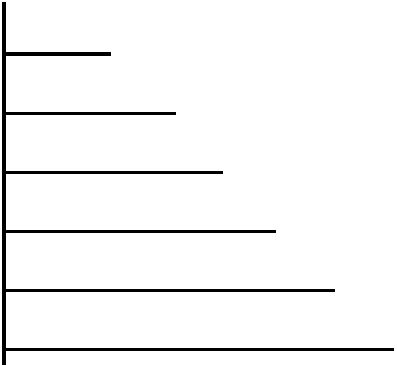
\includegraphics[width=0.36\textwidth]{gesamttex/edit_VIII,3/images/LH_35_09_14_001-002_d2.pdf}}%
  \vspace*{1.0em}
  \centerline{\lbrack\textit{Fig.~2}\rbrack}%
  \label{LH_35_09_14_002v_Fig.2}%
 %  \newpage%
%
%
% Ende des Textes